\section{Actividad No 01 – 	PRIMER LATEX AGREGADO} 

 \textbf{¿Qué buscan los sistemas de control de versiones?}
Gestionar ágilmente proyectos. Parte de su principal propósito es que puedas regresar a un estado anterior del proyecto o conocer, incluso, toda su evolución en el tiempo. Desde sus inicios hasta donde se encuentra actualizado. Puedes ver a los SCV como máquinas del tiempo, que permiten regresar a cualquier momento que quieras de tu proyecto. 

\begin{center}
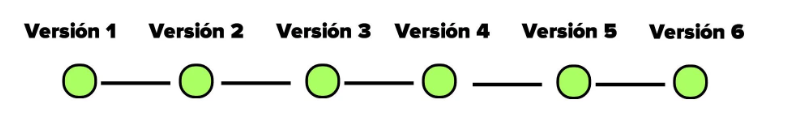
\includegraphics[width=10cm]{./Imagenes/Imagen001.png} 
\end{center}

Imagina el proyecto de Mestros del Web. El primer lanzamiento es una versión funcional del sitio web. Pero muy tranquilo. Conforme han avanzado los años, se posiciona y ha llegado a una 6ª versión donde ha mejorado en todas sus perspectivas. Si un desarrollador nuevo quisiera ver el trabajo y la evolución durante todos estos años, si se utilizó Git desde el inicio, lo podrá ver sin ningún problema. Cada versión incluye mejoras en el código, imágenes, organización de carpetas, etc. El repositorio (historial) creado por Git, guarda TODO. Es como ver un libro de tu proyecto. Hagamos otra analogía, tenemos el famoso CTRL + Z. Cuando trabajas en Word, sabemos que hay momentos donde necesitas regresar a un momento anterior (porque te equivocaste, etc.). Su historial temporal permite manejarte ágilmente con los errores. Los SCV persiguen el mismo objetivo. La diferencia es que éstos tienen un ecosistema para que puedas gestionar cada cambio de la mejor manera.